\documentclass{standalone}
\usepackage{tikz}
\usepackage{tikz-qtree}
\usepackage[makeroom]{cancel}
\usetikzlibrary{fit}

% ОПИСАНИЕ: модификация старого алгоритма tree overlap чтобы покрывать все деревья 
\begin{document} 
	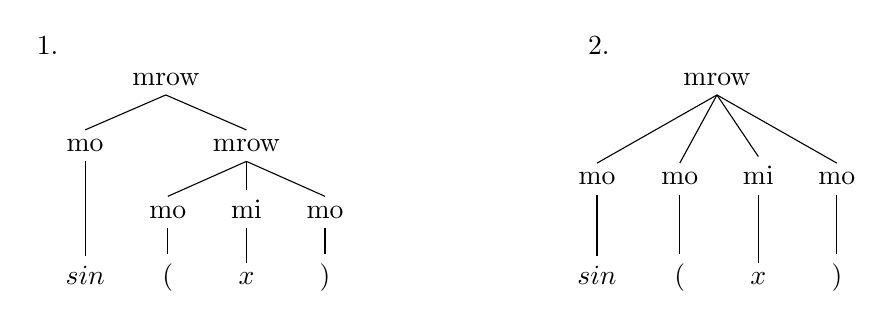
\begin{tikzpicture}[sibling distance=9.5pt]
	\tikzset{every tree node/.style={align=center,anchor=base}}
	\tikzset{level 1+/.style={level distance=2\baselineskip}}
	\tikzset{frontier/.style={distance from root=6\baselineskip}}

	\node (x) at (-1.5,0.5) {$1.$};
	    \Tree [.mrow
	            [.mo
	                $sin$  ] 
	            [.mrow
	                [.mo $($ ]
	                [.mi $x$ ]
	                [.mo $)$ ] ]]
	    \begin{scope}[xshift=7cm]
	\tikzset{level 1+/.style={level distance=3\baselineskip}}
	\node (y) at (-1.5,0.5) {$2.$};
	    \Tree [.mrow 
	                [.mo $sin$ ] 
	                [.mo $($ ] 
	                [.mi $x$ ] 
	                [.mo $)$ ]]
	    \end{scope}
	\end{tikzpicture}
\end{document} 